% Options for packages loaded elsewhere
\PassOptionsToPackage{unicode}{hyperref}
\PassOptionsToPackage{hyphens}{url}
\PassOptionsToPackage{dvipsnames,svgnames,x11names}{xcolor}
%
\documentclass[
  twocolumn,
  landscape]{report}

\usepackage{amsmath,amssymb}
\usepackage{iftex}
\ifPDFTeX
  \usepackage[T1]{fontenc}
  \usepackage[utf8]{inputenc}
  \usepackage{textcomp} % provide euro and other symbols
\else % if luatex or xetex
  \usepackage{unicode-math}
  \defaultfontfeatures{Scale=MatchLowercase}
  \defaultfontfeatures[\rmfamily]{Ligatures=TeX,Scale=1}
\fi
\usepackage[]{libertinus}
\ifPDFTeX\else  
    % xetex/luatex font selection
\fi
% Use upquote if available, for straight quotes in verbatim environments
\IfFileExists{upquote.sty}{\usepackage{upquote}}{}
\IfFileExists{microtype.sty}{% use microtype if available
  \usepackage[]{microtype}
  \UseMicrotypeSet[protrusion]{basicmath} % disable protrusion for tt fonts
}{}
\makeatletter
\@ifundefined{KOMAClassName}{% if non-KOMA class
  \IfFileExists{parskip.sty}{%
    \usepackage{parskip}
  }{% else
    \setlength{\parindent}{0pt}
    \setlength{\parskip}{6pt plus 2pt minus 1pt}}
}{% if KOMA class
  \KOMAoptions{parskip=half}}
\makeatother
\usepackage{xcolor}
\usepackage[top=30mm,left=20mm,heightrounded]{geometry}
\setlength{\emergencystretch}{3em} % prevent overfull lines
\setcounter{secnumdepth}{-\maxdimen} % remove section numbering
% Make \paragraph and \subparagraph free-standing
\ifx\paragraph\undefined\else
  \let\oldparagraph\paragraph
  \renewcommand{\paragraph}[1]{\oldparagraph{#1}\mbox{}}
\fi
\ifx\subparagraph\undefined\else
  \let\oldsubparagraph\subparagraph
  \renewcommand{\subparagraph}[1]{\oldsubparagraph{#1}\mbox{}}
\fi


\providecommand{\tightlist}{%
  \setlength{\itemsep}{0pt}\setlength{\parskip}{0pt}}\usepackage{longtable,booktabs,array}
\usepackage{calc} % for calculating minipage widths
% Correct order of tables after \paragraph or \subparagraph
\usepackage{etoolbox}
\makeatletter
\patchcmd\longtable{\par}{\if@noskipsec\mbox{}\fi\par}{}{}
\makeatother
% Allow footnotes in longtable head/foot
\IfFileExists{footnotehyper.sty}{\usepackage{footnotehyper}}{\usepackage{footnote}}
\makesavenoteenv{longtable}
\usepackage{graphicx}
\makeatletter
\def\maxwidth{\ifdim\Gin@nat@width>\linewidth\linewidth\else\Gin@nat@width\fi}
\def\maxheight{\ifdim\Gin@nat@height>\textheight\textheight\else\Gin@nat@height\fi}
\makeatother
% Scale images if necessary, so that they will not overflow the page
% margins by default, and it is still possible to overwrite the defaults
% using explicit options in \includegraphics[width, height, ...]{}
\setkeys{Gin}{width=\maxwidth,height=\maxheight,keepaspectratio}
% Set default figure placement to htbp
\makeatletter
\def\fps@figure{htbp}
\makeatother

\usepackage{booktabs}
\usepackage{longtable}
\usepackage{array}
\usepackage{multirow}
\usepackage{wrapfig}
\usepackage{float}
\usepackage{colortbl}
\usepackage{pdflscape}
\usepackage{tabu}
\usepackage{threeparttable}
\usepackage{threeparttablex}
\usepackage[normalem]{ulem}
\usepackage{makecell}
\usepackage{xcolor}
\makeatletter
\makeatother
\makeatletter
\makeatother
\makeatletter
\@ifpackageloaded{caption}{}{\usepackage{caption}}
\AtBeginDocument{%
\ifdefined\contentsname
  \renewcommand*\contentsname{Table of contents}
\else
  \newcommand\contentsname{Table of contents}
\fi
\ifdefined\listfigurename
  \renewcommand*\listfigurename{List of Figures}
\else
  \newcommand\listfigurename{List of Figures}
\fi
\ifdefined\listtablename
  \renewcommand*\listtablename{List of Tables}
\else
  \newcommand\listtablename{List of Tables}
\fi
\ifdefined\figurename
  \renewcommand*\figurename{Figure}
\else
  \newcommand\figurename{Figure}
\fi
\ifdefined\tablename
  \renewcommand*\tablename{Table}
\else
  \newcommand\tablename{Table}
\fi
}
\@ifpackageloaded{float}{}{\usepackage{float}}
\floatstyle{ruled}
\@ifundefined{c@chapter}{\newfloat{codelisting}{h}{lop}}{\newfloat{codelisting}{h}{lop}[chapter]}
\floatname{codelisting}{Listing}
\newcommand*\listoflistings{\listof{codelisting}{List of Listings}}
\makeatother
\makeatletter
\@ifpackageloaded{caption}{}{\usepackage{caption}}
\@ifpackageloaded{subcaption}{}{\usepackage{subcaption}}
\makeatother
\makeatletter
\@ifpackageloaded{tcolorbox}{}{\usepackage[skins,breakable]{tcolorbox}}
\makeatother
\makeatletter
\@ifundefined{shadecolor}{\definecolor{shadecolor}{rgb}{.97, .97, .97}}
\makeatother
\makeatletter
\makeatother
\makeatletter
\makeatother
\ifLuaTeX
  \usepackage{selnolig}  % disable illegal ligatures
\fi
\IfFileExists{bookmark.sty}{\usepackage{bookmark}}{\usepackage{hyperref}}
\IfFileExists{xurl.sty}{\usepackage{xurl}}{} % add URL line breaks if available
\urlstyle{same} % disable monospaced font for URLs
\hypersetup{
  pdftitle={LABORATÓRIO 1: Relação da concentração de glicose no plasma com características diversas},
  pdfauthor={Fernando Bispo, Jeff Caponero},
  colorlinks=true,
  linkcolor={blue},
  filecolor={Maroon},
  citecolor={Blue},
  urlcolor={Blue},
  pdfcreator={LaTeX via pandoc}}

\title{LABORATÓRIO 1: Relação da concentração de glicose no plasma com
características diversas}
\author{Fernando Bispo, Jeff Caponero}
\date{}

\begin{document}
\maketitle
\ifdefined\Shaded\renewenvironment{Shaded}{\begin{tcolorbox}[boxrule=0pt, frame hidden, interior hidden, enhanced, borderline west={3pt}{0pt}{shadecolor}, breakable, sharp corners]}{\end{tcolorbox}}\fi

\listoffigures
\listoftables
\hypertarget{apresentauxe7uxe3o}{%
\section{Apresentação}\label{apresentauxe7uxe3o}}

Este relatório visa a descrição da análise realizada nos dados oriundos
do Instituto Nacional de Diabetes e de Doenças Digestivas e Renais dos
EUA que conduziram um estudo com 768 mulheres da tribo Pina, que residem
próximo a Phoenix e coletaram as seguintes características das
participantes do estudo:

\begin{itemize}
\tightlist
\item
  Número de gestações {[}\textbf{pregnat}{]};
\item
  Concentração de glicose no plasma (obtido duas horas depois da
  realização de um teste de tolerância a glicose)
  {[}\textbf{glucose}{]}; pressão sanguínea diastólica (mmHg)
  {[}\textbf{diastolic}{]};
\item
  Largura do tríceps (mm) {[}\textbf{triceps}{]};
\item
  Nível de insulina (µU/ml) {[}\textbf{insulin}{]};
\item
  Índice de massa corpórea (kg/m2) {[}\textbf{bmi}{]};
\item
  Nível de função diabética {[}\textbf{diabetes}{]};
\item
  Iidade em anos {[}\textbf{age}{]};
\item
  Teste para avaliação de sinais de diabetes (0 = negativo e 1 =
  positivo) {[}\textbf{teste}{]}.
\end{itemize}

\hypertarget{anuxe1lise-descritiva}{%
\section{Análise Descritiva}\label{anuxe1lise-descritiva}}

\subsection{Dados sem tratamento}

Neste primeiro momento será realizada a análise das características sem
nenhum tipo de tratativa dos dados, a fim de identificar padrões,
partindo, a princípio, da tabela contendo as principais medidas de
posição e dispersão.

\begin{table}

\caption{\label{tab:unnamed-chunk-2}Tabela 1: Medidas Resumo}
\centering
\begin{tabu} to \linewidth {>{\raggedright}X>{\centering}X>{\centering}X>{\centering}X>{\centering}X>{\centering}X>{\centering}X>{\centering}X>{\centering}X}
\hline
  & Min & Q1 & Med & Média & Q3 & Max & D.Padrão & CV\\
\hline
\cellcolor{TRUE}{Glicose} & \cellcolor{TRUE}{0,00} & \cellcolor{TRUE}{99,00} & \cellcolor{TRUE}{117,00} & \cellcolor{TRUE}{120,89} & \cellcolor{TRUE}{140,50} & \cellcolor{TRUE}{199,00} & \cellcolor{TRUE}{31,97} & \cellcolor{TRUE}{0,26}\\
\hline
Idade & 21,00 & 24,00 & 29,00 & 33,24 & 41,00 & 81,00 & 11,76 & 0,35\\
\hline
\cellcolor{TRUE}{IMC} & \cellcolor{TRUE}{0,00} & \cellcolor{TRUE}{27,30} & \cellcolor{TRUE}{32,00} & \cellcolor{TRUE}{31,99} & \cellcolor{TRUE}{36,60} & \cellcolor{TRUE}{67,10} & \cellcolor{TRUE}{7,88} & \cellcolor{TRUE}{0,25}\\
\hline
Largura Triceps & 0,00 & 0,00 & 23,00 & 20,54 & 32,00 & 99,00 & 15,95 & 0,78\\
\hline
\cellcolor{TRUE}{N° de Gestações} & \cellcolor{TRUE}{0,00} & \cellcolor{TRUE}{1,00} & \cellcolor{TRUE}{3,00} & \cellcolor{TRUE}{3,85} & \cellcolor{TRUE}{6,00} & \cellcolor{TRUE}{17,00} & \cellcolor{TRUE}{3,37} & \cellcolor{TRUE}{0,88}\\
\hline
Nivel Diabético & 0,08 & 0,24 & 0,37 & 0,47 & 0,63 & 2,42 & 0,33 & 0,70\\
\hline
\cellcolor{TRUE}{Nível Insulina} & \cellcolor{TRUE}{0,00} & \cellcolor{TRUE}{0,00} & \cellcolor{TRUE}{30,50} & \cellcolor{TRUE}{79,80} & \cellcolor{TRUE}{127,50} & \cellcolor{TRUE}{846,00} & \cellcolor{TRUE}{115,24} & \cellcolor{TRUE}{1,44}\\
\hline
P. Diastólica & 0,00 & 62,00 & 72,00 & 69,11 & 80,00 & 122,00 & 19,36 & 0,28\\
\hline
\multicolumn{9}{l}{\rule{0pt}{1em}\textit{Note: }}\\
\multicolumn{9}{l}{\rule{0pt}{1em}Fonte: Instituto Nacional de Diabetes e de Doenças Digestivas e Renais - EUA}\\
\end{tabu}
\end{table}

Conforme consta na Figura 1, cerca de 35\% das participantes
apresentaram resultado positivo para a presença de sinais de diabetes.

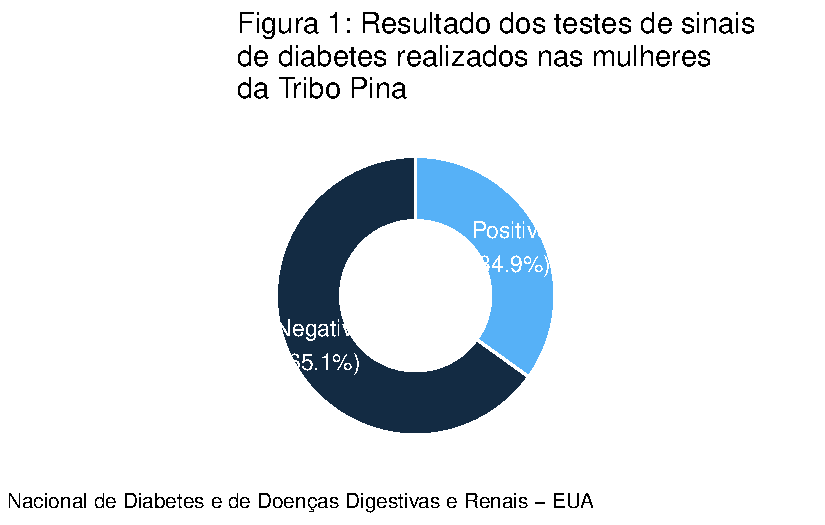
\includegraphics{relatorio_lab1_files/figure-pdf/unnamed-chunk-3-1.pdf}

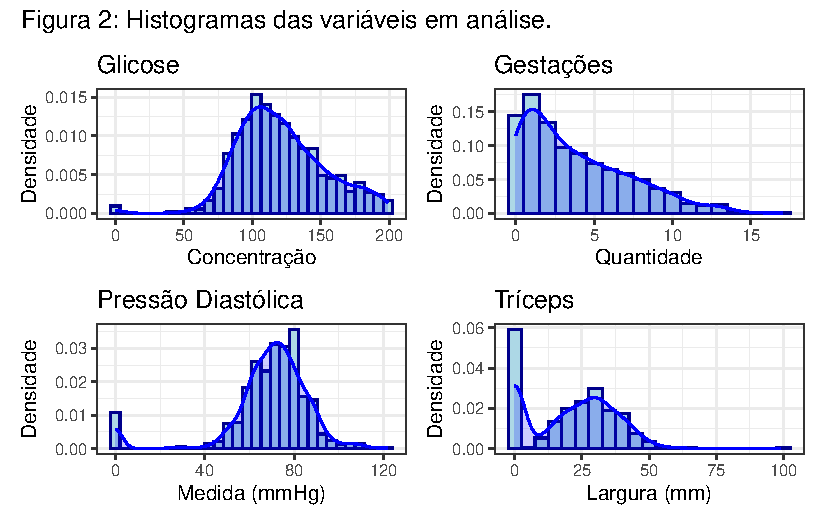
\includegraphics{relatorio_lab1_files/figure-pdf/unnamed-chunk-4-1.pdf}

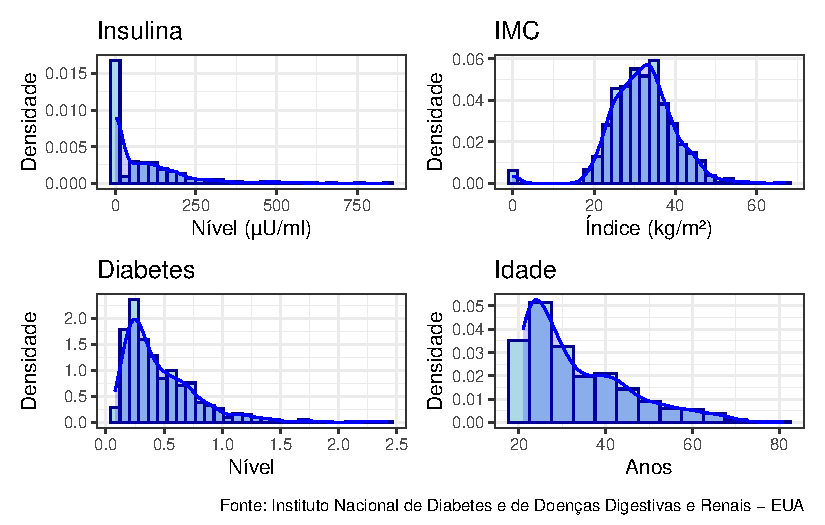
\includegraphics{relatorio_lab1_files/figure-pdf/unnamed-chunk-4-2.pdf}

A fim de avaliar a correlação entre a variável de interesse (Nível de
Diabetes) com as demais variáveis, foram construídos gráficos de
dispersão para realização desta avaliação.

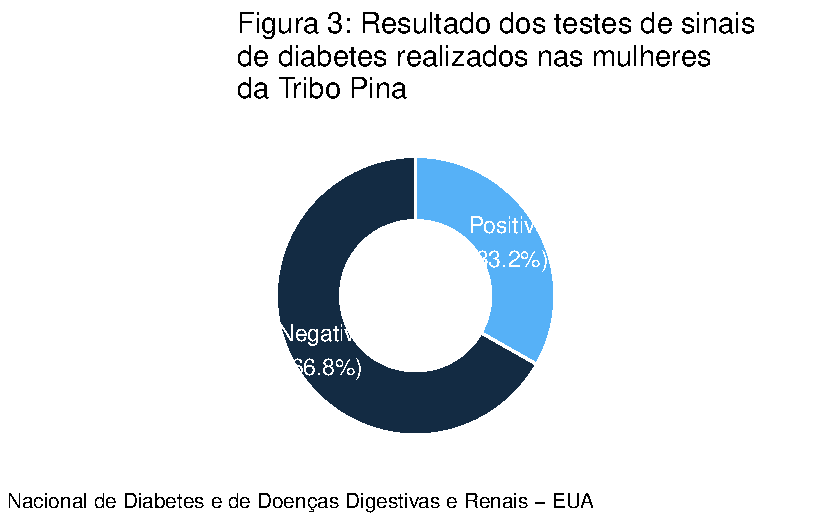
\includegraphics{relatorio_lab1_files/figure-pdf/unnamed-chunk-6-1.pdf}

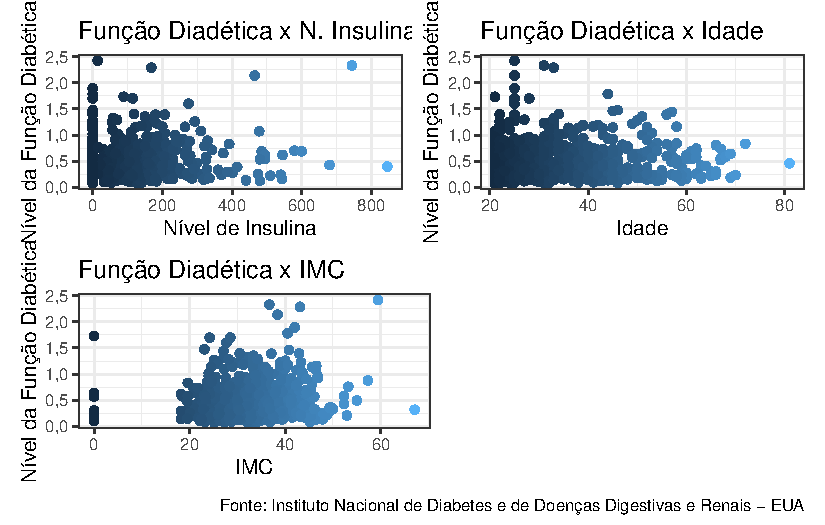
\includegraphics{relatorio_lab1_files/figure-pdf/unnamed-chunk-6-2.pdf}

\subsection{Dados tratados}

\begin{table}

\caption{\label{tab:unnamed-chunk-7}Tabela 2: Medidas Resumo}
\centering
\begin{tabular}[t]{l|c|c|c|c|c|c|c|c}
\hline
  & Min & Q1 & Med & Média & Q3 & Max & D. Padrão & CV\\
\hline
\cellcolor{TRUE}{Glicose} & \cellcolor{TRUE}{56,00} & \cellcolor{TRUE}{99,00} & \cellcolor{TRUE}{119,00} & \cellcolor{TRUE}{122,63} & \cellcolor{TRUE}{143,00} & \cellcolor{TRUE}{198,00} & \cellcolor{TRUE}{30,86} & \cellcolor{TRUE}{0,25}\\
\hline
Idade & 21,00 & 23,00 & 27,00 & 30,86 & 36,00 & 81,00 & 10,20 & 0,33\\
\hline
\cellcolor{TRUE}{IMC} & \cellcolor{TRUE}{18,20} & \cellcolor{TRUE}{28,40} & \cellcolor{TRUE}{33,20} & \cellcolor{TRUE}{33,09} & \cellcolor{TRUE}{37,10} & \cellcolor{TRUE}{67,10} & \cellcolor{TRUE}{7,03} & \cellcolor{TRUE}{0,21}\\
\hline
Largura Triceps & 7,00 & 21,00 & 29,00 & 29,15 & 37,00 & 63,00 & 10,52 & 0,36\\
\hline
\cellcolor{TRUE}{N° de Gestações} & \cellcolor{TRUE}{0,00} & \cellcolor{TRUE}{1,00} & \cellcolor{TRUE}{2,00} & \cellcolor{TRUE}{3,30} & \cellcolor{TRUE}{5,00} & \cellcolor{TRUE}{17,00} & \cellcolor{TRUE}{3,21} & \cellcolor{TRUE}{0,97}\\
\hline
Nivel Diabético & 0,09 & 0,27 & 0,45 & 0,52 & 0,69 & 2,42 & 0,35 & 0,66\\
\hline
\cellcolor{TRUE}{Nível Insulina} & \cellcolor{TRUE}{14,00} & \cellcolor{TRUE}{76,50} & \cellcolor{TRUE}{125,50} & \cellcolor{TRUE}{156,06} & \cellcolor{TRUE}{190,00} & \cellcolor{TRUE}{846,00} & \cellcolor{TRUE}{118,84} & \cellcolor{TRUE}{0,76}\\
\hline
P. Diastólica & 24,00 & 62,00 & 70,00 & 70,66 & 78,00 & 110,00 & 12,50 & 0,18\\
\hline
\multicolumn{9}{l}{\rule{0pt}{1em}\textit{Note: }}\\
\multicolumn{9}{l}{\rule{0pt}{1em}Fonte: Instituto Nacional de Diabetes e de Doenças Digestivas e Renais - EUA}\\
\end{tabular}
\end{table}

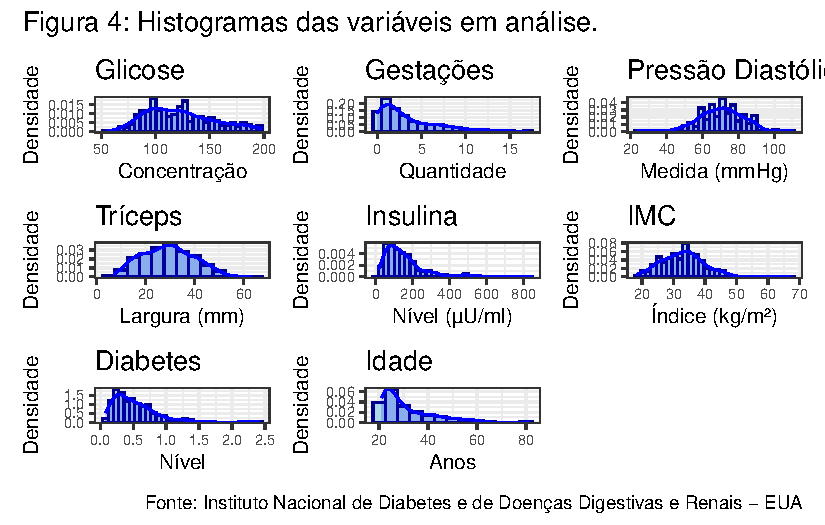
\includegraphics{relatorio_lab1_files/figure-pdf/unnamed-chunk-8-1.pdf}

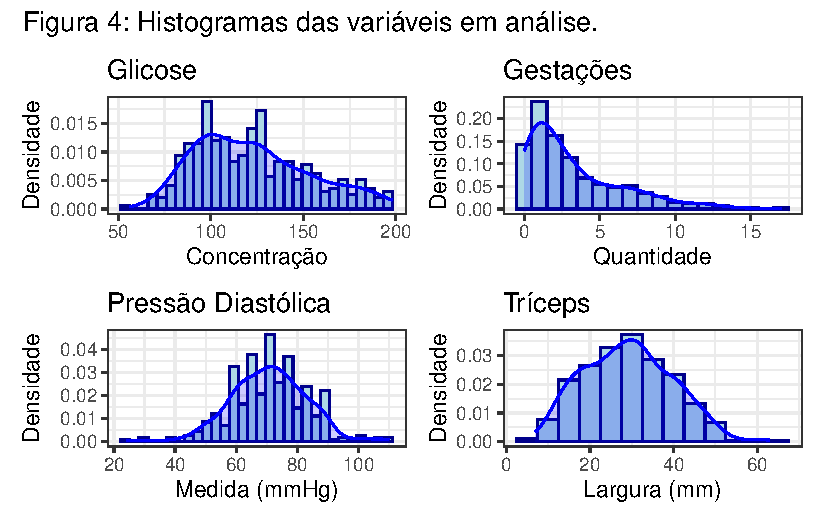
\includegraphics{relatorio_lab1_files/figure-pdf/unnamed-chunk-10-1.pdf}

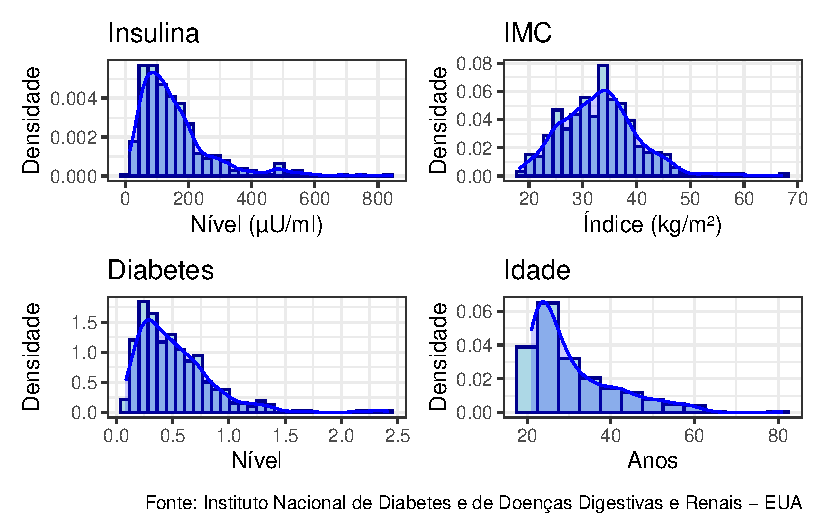
\includegraphics{relatorio_lab1_files/figure-pdf/unnamed-chunk-10-2.pdf}

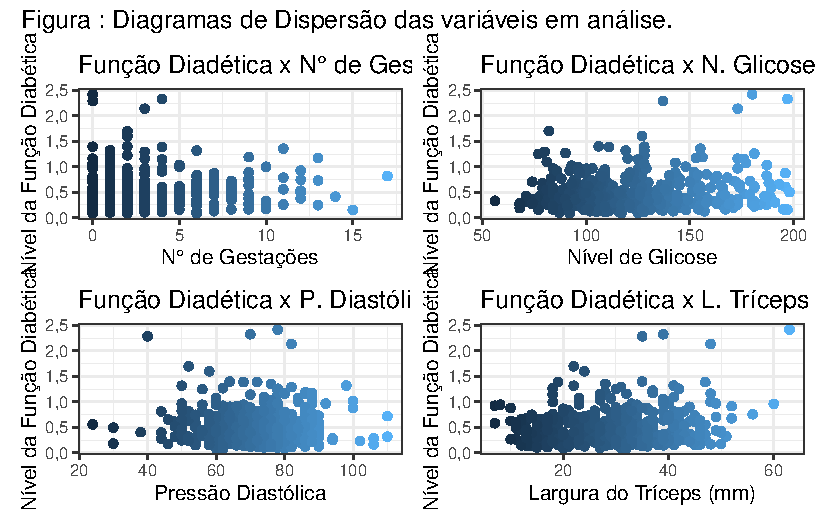
\includegraphics{relatorio_lab1_files/figure-pdf/unnamed-chunk-11-1.pdf}

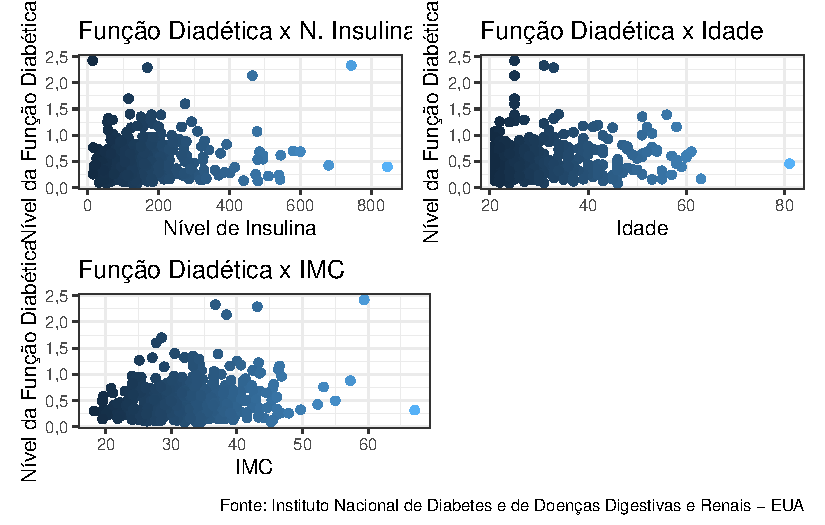
\includegraphics{relatorio_lab1_files/figure-pdf/unnamed-chunk-11-2.pdf}

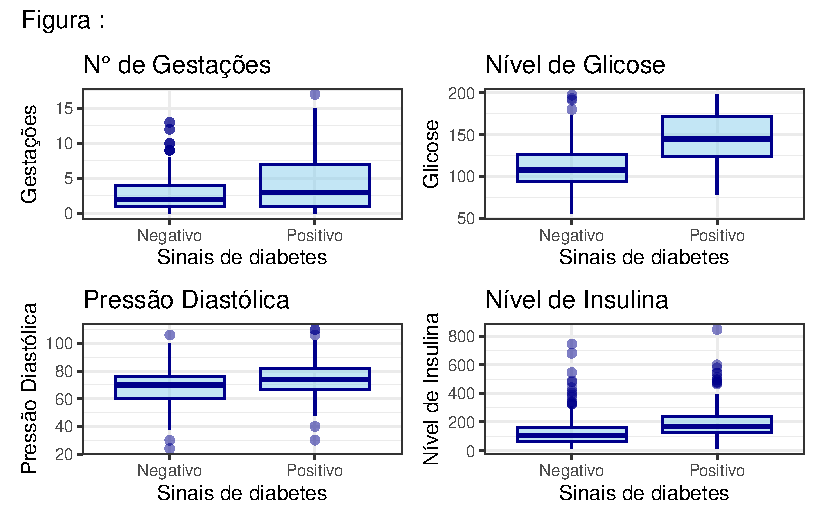
\includegraphics{relatorio_lab1_files/figure-pdf/unnamed-chunk-12-1.pdf}

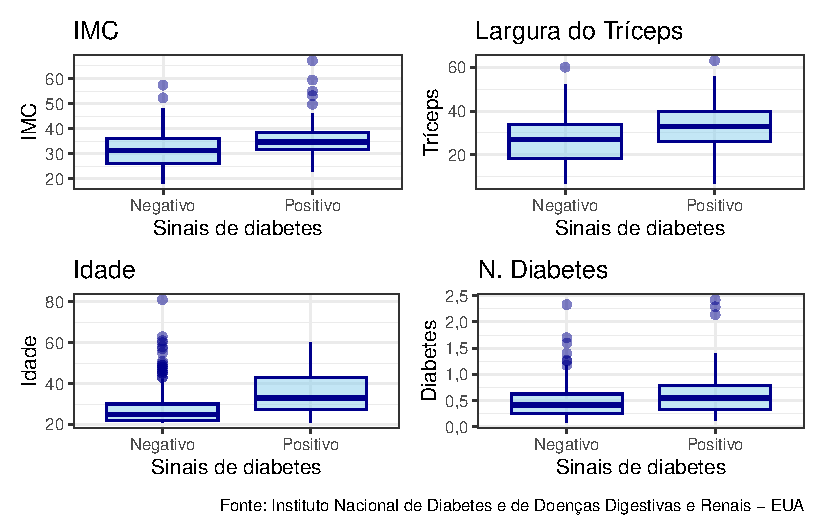
\includegraphics{relatorio_lab1_files/figure-pdf/unnamed-chunk-12-2.pdf}

\hypertarget{conclusuxe3o}{%
\section{Conclusão}\label{conclusuxe3o}}



\end{document}
